\section{Construction}\label{sec:construction}

\begin{figure*}
    \centering
    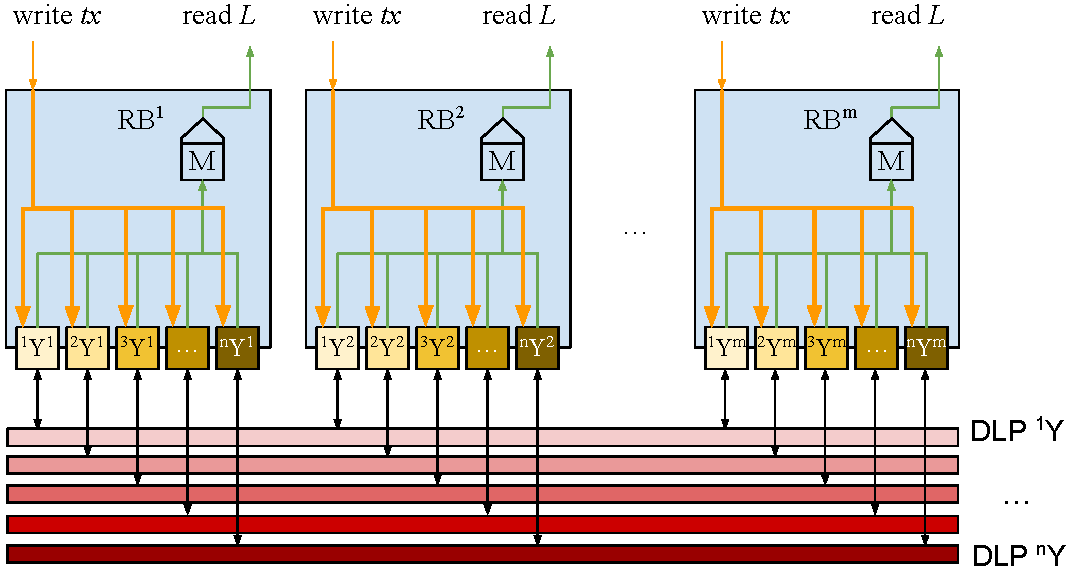
\includegraphics[width=\textwidth,keepaspectratio]{figures/rollerblade-naive-construction.pdf}
    \caption{The first attempt at the composed construction. Here,
             $m$ different parties $\RB_1, \ldots, \RB_m$ operate Rollerblade
             nodes, each of which runs a client on $n$ different underlying
             DLPs $Y_1, \ldots, Y_n$.}
    \label{fig.naive}
\end{figure*}

\subsection{A Majority Vote}\label{sec:construction-naive}

In Figure~\ref{fig.naive}, $m$ parties $\RB_1, \ldots, \RB_m$ run the overlay protocol.
No honesty assumptions are made among the $\RB$ population. Each of the $\RB$ nodes runs
a full node to each of the $n$ underlying DLPs $Y_1, \ldots, Y_n$, pictured as squares
of varying shades of yellow. The full nodes communicate with one another using their
respective DLP technology, which we treat as a black box here, depicted as elongated
rectangles in varying shades of red towards the bottom of the figure. The $\RB$ nodes
make their own overlay DLP, offering \emph{read} and \emph{write} functionalities.
When an $\RB$ transaction $\tx$ is \emph{written} into one of the $\RB$ nodes by the user,
the $\RB$ serializes this transaction for each of the underlying DLPs (using the
serialization mechanism particular to each individual DLP) and posts it
as a transaction there, depicted as orange wires running downwards. Each of the
full nodes then propagates this transaction using its own DLP technology to the
other full nodes. For example, if the underlying $Y_1$ DLP is secure, then
the full node $Y_1$ running within $\RB_2$ will eventually see the transaction
posted by $\RB_1$ into its own $Y_1$ box. When the $\RB$ user requests to read the
ledger of the respective $\RB$ node, the node invokes the respective \emph{read}
functionality of all of its full node boxes, depicted as green wires running upwards
in the figure. The output of this \emph{read} operation is then filtered and deserialized
(using the deserialization mechanism particular to each individual DLP), then fed into a
\emph{majority voting} contraption, denoted with the letter M and the \emph{house} symbol
in the figure, which then outputs the desired ledger $L$ of $\RB$ transactions.

\subsection{A BFT to Rule Them All}\label{sec:construction-bft}

\begin{itemize}
  \item DLP protocols. ``Read'' ledger and ``write'' tx functionalities (temporal ledgers?). Safety and liveness ($u$), security definitions.
  \item Simple majority voting construction with no BFT protocol on top. Serialization and deserialization requirements and algorithms. Majority voting on ``ledger extensions'' algorithm. Fragile results in which different blockchains can disagree on the order and one blockchain can ``flip over'' the result. l. Condorcet cycles.
  \item The necessity of running a BFT protocol on top, but without talking about the oracle abstraction of signatures, broadcasting, verification, and receiving. Light clients from one blockchain to another using smart contracts. Using the blockchains as ports of communication.
  \item Oraclizing sign/broadcast and receive/verify.
  \item Remove the smart contract assumption using dirty ledgers.
  \item The full construction.
\end{itemize}

\subsection{Compatibility}\label{sec:compatibility}

\import{./}{algorithms/alg-rollerblade}
\import{./}{algorithms/alg-majorityvote}
\import{./}{algorithms/alg-relay}
\import{./}{algorithms/alg-view}
\import{./}{algorithms/alg-simulate}
\import{./}{algorithms/alg-encode}
\import{./}{algorithms/alg-ledger}
